\documentclass[i2]{oss}
\setlength{\topmargin}{-.5in}
\setlength{\textheight}{9in}
\setlength{\oddsidemargin}{.100in}
\setlength{\textwidth}{6.25in}
\usepackage[english]{babel}
\usepackage{graphicx}
\usepackage{amsmath}
\usepackage{fullpage}
\usepackage{color}
\usepackage{soul}
%\usepackage{gensymb}
\usepackage{caption}
\usepackage{subcaption}
\usepackage[section]{placeins}
\usepackage{parskip}

\newcommand{\class}[1]{\emph{#1}}
\newcommand{\method}[1]{\emph{#1}}
\newcommand{\junit}{\emph{JUnit }}
\newcommand{\comment}[1]{{\huge \textcolor{green}{#1}}\\}

\begin{document}

\members{Joren Verspeurt {\small \texttt{(r0258417)} } \\ %# Commentaar
         Sophie Marien {\small \texttt{(s0216517)}}\\
         Stef Noten {\small \texttt{(s0211264)}}\\
         Toon Nolten {\small \texttt{(r0258654)}} \\
         Begeleider: Mario H. C. T.} % teamleden

\maketitlepage
\newpage
\tableofcontents
\pagebreak




%-----------------------------------------------------------------------
%	INLEIDING
%-----------------------------------------------------------------------
\section*{Introduction}
\label{ssec:introduction}
%introductie en de belangrijkste elementen van ons ontwerp

Unit Tests are important because today's software systems are very 
complex.
\junit is the most popular framework for unit testing in the Java 
language.
Currently running the tests is either done manually by developers or
automatically by a continuous integration tool on a central server.
A disadvantage of these approaches is that tests only run when a 
developer decides to or when a developer commits work to the central 
repository.
This can be improved by using a daemon (background process) that continuously runs tests, this gives the developer rapid feedback and 
takes away the burden of manually starting tests.

%-----------------------------------------------------------------------
%	ALGEMENE BESLISSINGEN
%-----------------------------------------------------------------------
\section{General decisions}
\label{ssec:general-decisions}

A new testrun should be executed when source code changes, either in tests or in classes that are being tested. 
A granularity of picked up changes has to be chosen.
A distinction between code changes in different classes should obviously be made.
It is however not immediately clear at which granularity changes inside a class should be detected.
Changes in methods could be detected separately.
Even a distinction between different execution paths inside a method could be made.
However, we argue that a class should be coherent and as such, a change of the code of a method would have a high possibility of impacting the behaviour of the whole class.
Therefore, code changes will be looked at only at the level of classes and a finer distinction will not be made.

Changes to the classes will be detected by monitoring their *.class files.
An alternative would be to monitor the actual *.java source files, but most integrated development environments already offer automatic building functionality.
Moreover, the test daemon would have to know the specifics of how to compile the entire project. 
Therefore, it will be required that users of the automatic test daemon use the automatic building feature of their IDE.
The test daemon will pick up changes in the compiled *.class files and as a result, it will queue a new testrun.

Testruns should always always be executed completely.
Otherwise, when a developer is constantly making changes to the code, some tests would only be executed after a very long time.
Only when the developer would eventually take a break longer than the duration of a testrun, these tests would be executed.
While it could be argued that this is acceptable for some tests that are scheduled by a policy to run at the very end of a testrun, there are significant drawbacks to this approach.

An important drawback is starvation. Some policies can only change the execution order based on new information of runs of the tests.
This would mean that for tests that are initially scheduled at the very end, it would be very hard to raise their priority, even though some code changes could significantly affect their test result.
Even though techniques as aging could partially solve this starvation problem, the root of this problem would still be the same: new information on these tests is simply not available. Another solution would be to discard new information on all tests when the testrun has not completed entirely. However, this would undermine the purpose of the policy, since it could take very long until a policy would take new information into account.

Sometimes, a comparison between tests that are run more often and tests that starve at the end of the testrun, wouldn't even make sense.
Consider the priority of tests under the frequent failure first policy.
It is not clear how to do a fair comparison between tests under this policy when different tests are run more often than others.

Because of these reasons, when a testrun is executed, it will execute all the tests and leave no single one out.

\comment{Nog algemene beslissingen?}

%-----------------------------------------------------------------------
%	ONTWERP
%-----------------------------------------------------------------------
\section{Design}
\label{ssec:design}
%Klassendiagram en interactie diagrammen

In this section we describe how our design followed from an analysis
of responsibilities and we go through the start-up and execution of 
our application.

\subsection{Design overview and responsibilities}

The guiding principle for our design is a clear separation of 
responsibilities. The first step is an analysis of necessary actions:

\begin{itemize}
	\item Run tests
    \item Collect information on tests
    \item Summarize the available information for a test
    \item Order tests according to a user-specified policy
    \item Output of results
\end{itemize}

Each of these is different enough to merit an entire entity responsible 
for that action. Those entities were implemented as \class{Daemon},
\class{DataCollector}, \class{Statistic}, \class{Policy} and
\class{ConsoleView} respectively. Our daemon makes as much use of the 
existing \junit infrastructure as possible. 
%Stef: Misschien eerder eerst de belangrijke zaken uitleggen en deze details pas later vermelden?
We only needed to extend three existing classes: \class{FlattenedRequest}
is a request that flattens all tests in an existing Request, so that it only contains test methods (no suites) as children. 
This class is mostly based on \class{MaxCore} in the \junit experimental package. 
However, it makes use of a custom runner: \class{MethodRunner}. 
This class was necessary because when sorting a \class{FlattenedRequest}, the description of the children was actually the
description of the testclass containing the method and not the method 
itself.
\class{RunNotificationSubscriber} does not extend anything from 
\junit but is used as a protection proxy so \class{Daemon} does not have 
to pass an actual \class{RunNotifier} which could be used to fire events 
(testRunStarted, testFailed...). 

The \class{Daemon} is responsible for executing testruns.
It can make use of different \class{Policy}'s to order the tests that 
need to be run. 

A \class{Policy} is responsible for transforming a \class{Request} into a \class{Request} that is run according to the rules of the \class{Policy}. 
These can be all different kinds of rules, but only policies that sort the executing tests have been implemented. 
An example of another possible rule is the filtering of requests.
%# Ik kon niet zo direct iets anders bedenken dat ze zouden kunnen doen maar als iemand nog ergens op komt schrijf het er bij.
The abstract \class{SortingPolicy} class implements a policy that can sort its executing test methods. It asks of its concrete classes only a comparator that determines an order between two \class{Description}s, which correspond to a test.
All implemented sorting policies make use of \class{Statistic}s to determine
an order for tests, but this is not required.
At the moment, the following policies are supported: last failure first, 
frequent failure first, distinct failure first and changed code 
first.
Each of these determines a different order that can be useful for
developers.
For example, tests that consistently order first under the frequent
%failure first policy might indicate brittle/(badly written) code.
failure first policy might indicate fragile / badly written code. 
%# Ik heb nog nooit het woord brittle gebruikt zien worden voor code, het klinkt een beetje vreemd, maar als ge zeker weet dat Mario gaat weten wat ge bedoelt zet het er maar bij
%-- Brittle betekent dat iets heel gemakkelijk breekt, iemand die engels spreekt zal dat wel begrijpen denk ik, slecht geschreven vindt ik een beetje teveel oordelend, misschien 'fragile'?
%# Ja ik weet wat brittle betekent. Ik vind het alleen vreemd om code broos te noemen. Breekbaar misschien maar broos slaagt echt nergens op.

%# Ik heb dit stuk een beetje herschikt, het is op dit moment nog een beetje kort voor een eigen subsubsectie maar we kunnen het eventueel afsplitsen als het te groot wordt.
To enable handling tests in different ways in response to different 
events that can occur during testing, \class{Statistic}'s calculate any 
necessary information for the ordering from data collected by dedicated 
\class{DataCollector}'s. %% welke events? misschien hier dieper op ingaan
Examples of data that has to be collected for the supported policies: 
every failure of a test, which code a test depends on and which code 
changes on disk during execution.
%# Verzoek voor goedkeuring volgend deel
The original design included a kind of data storage class where collected
data or statistics could be kept, but this generated too much coupling
and placed too much responsibility on this single class.
The structure was altered and in the current design a \class{Statistic}
only keeps the data that it needs.
%# idem
A \class{Policy} gains access to one or more \class{Statistic}'s through
the \class{StatisticProvider}.
A \class{Policy} sends the kind of statistic it needs to the 
\class{StatisticProvider}, which then responds with a \class{Statistic}
that can provide it if it knows about such a \class{Statistic}, otherwise
an exception is thrown.
This way a layer of indirection is created between \class{Policy}'s and
\class{Statistic}'s so another class that produces the same kind of 
statistic data as an existing \class{Statistic} but in a different way 
can easily substituted for that existing \class{Statistic}. 
It also enables sharing of different \class{Statistic}'s between 
\class{Policy}'s.
%# Zouden we hier ook iets bij zetten over dat alternatief design met de chain of responsibility van factories voor het aanmaken van Statistics?

%# Ook niet genoeg voor een eigen subsubsectie
%\subsubsection{Collecting data for statistics}
\class{DataCollector}'s are responsible for collecting necessary data 
during execution.
Some \class{DataCollector}'s collect data about tests that have been run,
some collect data about changes in the testing environment such as files that have been changed.
%# Hier misschien wat meer over hoe ze werken (als in met welke delen van junit etc. ze gekoppeld zijn en zo)
\class{DataCollector}'s are available through the \class{DataEnroller}
that provides the service of subscribing \class{Statistic}'s to specific
\class{DataCollector}'s.
%# TODO: meer informatie over design decisions over DataCollectors
\class{DataCollector}'s that gather information about tests currently
don't support parallel testing because this was not seen as a 
high-priority issue, \junit itself only supports parallel testing as an
experimental feature.



%# Mag dit dan weg?

%\begin{description}
%\item Collecting Statistics.( rejecting of the statistic pool)
%At the beginning of the brainstorm of the design we included a class {Statistic Pool}. This class would have kept all the statistics. By a request there will be checked if it owns a specific statistic. If the requested statistic is not owned by the \emph{StatisticPool} then the statistic will be registered. This was eventually rejected because there would be too much dependenty on this class. Statistics are still beeing kept but this is now done in the \emph{StatisticManager}.

%\item Policies
%Composite filters and sorting policies.
%A \emph{Policy} has an apply. This apply will operates on a request and it will return a request. In addition, every policy has a child as Policy. If an apply is called, then it will first call the apply of the child and after that it will call its own apply on the resulting request. We can not guarantee that the result is correct according to the multiple sorting policies that are done. SortingRequest can not be applied over multiple niveaus (if there is a filterRequest in between). The assumption we are making here is that the new sorting will wipe out the older sorting instead of putting it together.
%TODO dit was veranderd naar een ander ontwerp

%\item Collectors
%For \emph{FailureTraceCollector} are the parallel tests not suported. This is not supported because it will take a lot of time to implement it and there are other priorities.
%\end{description}

\subsubsection{Data collectors}

A \class{DataCollector} is responsible for collecting a certain type of information on tests.
It has to link this information to a certain \junit \class{Description}, which corresponds with a \junit test. 
When it has collected such a data item for a \class{Description}, it has to notify all interested parties of this event.
Therefore, it also has to keep track of its interested parties.
%# Tof, maar zou ge dit niet beter bij het deel hier boven bij schrijven of de tekst van daar naar hier verplaatsen of iets dergelijks?
%Stef: ja het zou kunnen dat daar iets bij moet of van daar naar hier, maar ik denk dat in deze "detailsectie" alles wel volledig moet zijn, niet? Dus dan moet het wel een klein beetje dubbele info zijn, hiervoor is het tenslotte een samenvatting van wat in deze sectie allemaal komt
%# Bwa we hoeven onszelf toch sowieso niet te herhalen? Maar inderdaad er zou wel wat van boven naar hier opgeschoven kunnen worden.

%Stef: TODO waarom generic + exact uitleggen hoe
\class{DataCollector}s are generic in the type of data they collect.

No assumptions should be made about who these interested parties are. The only thing a \class{DataCollector} should  know, is that it is a party that is interested in the event that is has collected a data item. This notification problem is a typical problem that can be solved by the Observer pattern.

%Stef: TODO Modifications to the Observer pattern: 
%- in the original observer pattern: interested parties are only notified of the change event, after which they themself will look for the new state
%- afscherming van de echte datacollectors via de dataenroller

%Stef: TODO werking van elke collectors


%-------------KLASSENDIAGRAMMA------------------------------------------
\subsection{Class diagrams}
\label{ssec:Klassendiagramma}


%figuur oud klassendiagram
\begin{figure}[tbp]
\begin{center}
    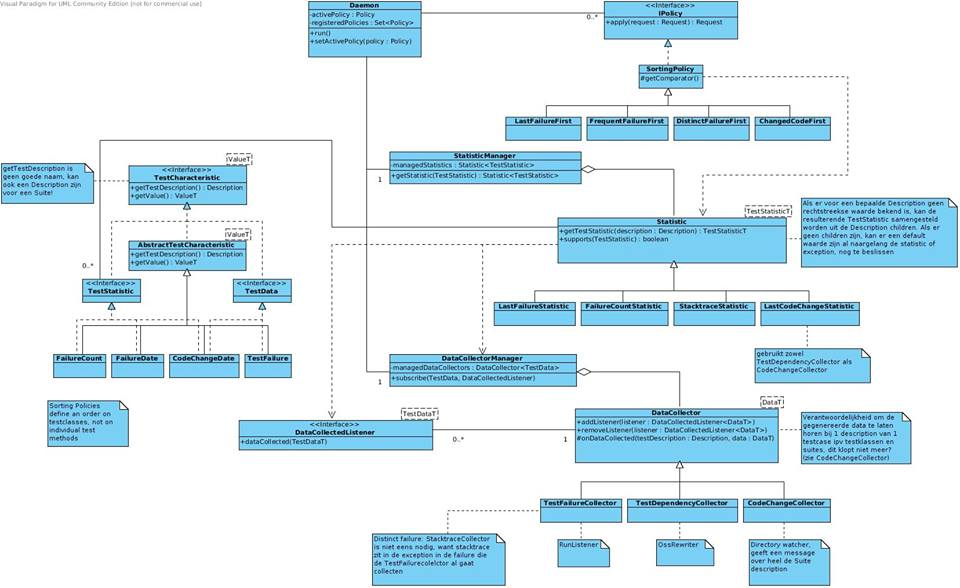
\includegraphics[width=0.8\textwidth]{klassendiagramOud}
    \caption{The old classdiagram}
	\label{fig:kd-oud}
\end{center}
\end{figure}



%figuur nieuw klassendiagram
\begin{figure}[tbp]
\begin{center}
    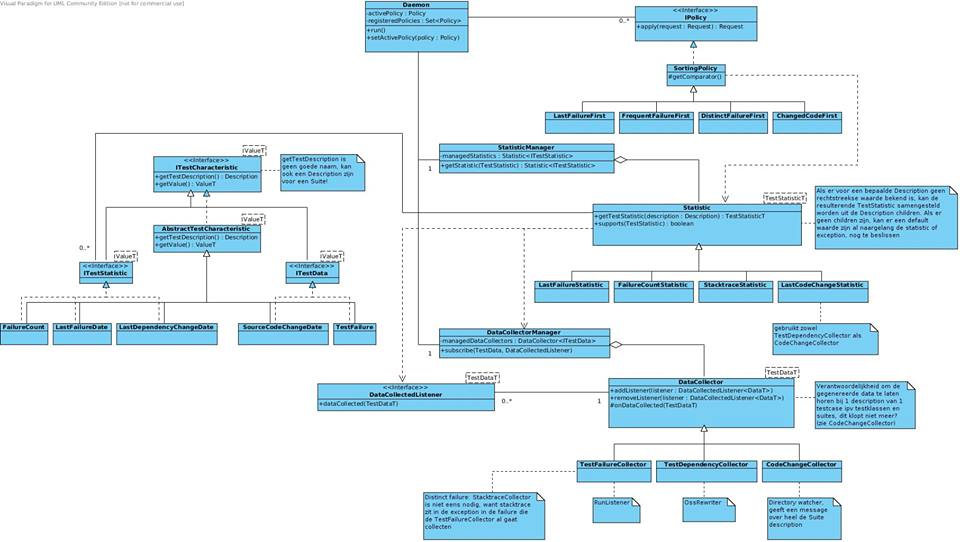
\includegraphics[width=0.8\textwidth]{klassendiagram}
    \caption{The intermediate classdiagram}
	\label{fig:kd-tt}
\end{center}
\end{figure}




%figuur nieuw klassendiagram
\begin{figure}[tbp]
\begin{center}
    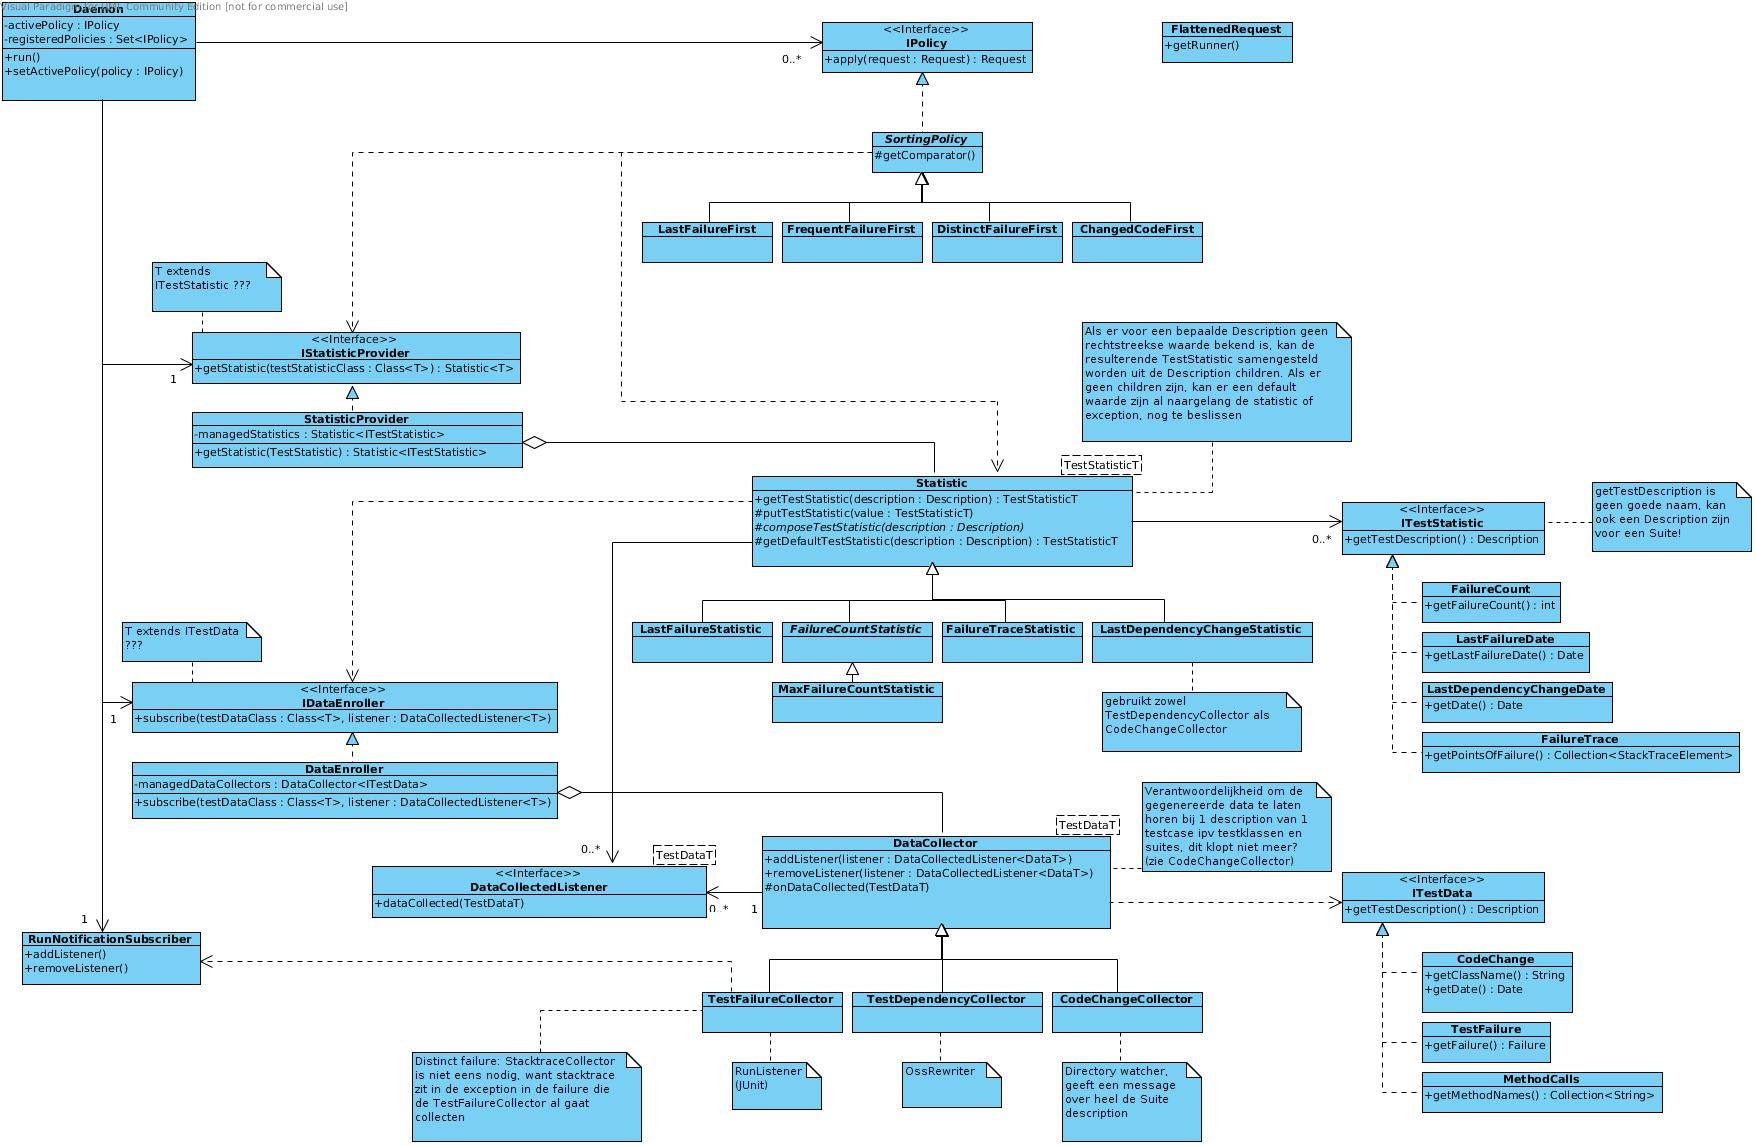
\includegraphics[width=0.8\textwidth]{klassendiagram3}
    \caption{Current classdiagram}
	\label{fig:kd-h}
\end{center}
\end{figure}



%-------------Interactie Diagrammas-------------------------------------
\subsection{Execution of the application}

%# TODO

\subsection{Interaction diagrams}
\label{ssec:Interactiedia}

%# TODO



%-----------------------------------------------------------------------
%	TESTEN
%-----------------------------------------------------------------------
\section{Tests}
\label{ssec:tests}

For testing the application a two-fold approach was used: unit tests for
important classes and a dummy project to use the application on.
%# Voor zo ver ik gezien heb gebruiken we niet echt mocks, mocks verzamelen intern ook gegevens over de tests (zo kan een methode bijhouden hoe veel keer die is opgeroepen en zo'n dingen) en bestaan uit meer dan alleen maar stubs van methoden die opgeroepen worden in de tests.
This dummy project includes some stub classes which contain methods that
exhibit behaviour that is interesting to test on.
For example there are classes that only include methods that throw 
exceptions.
There are also tests in this project that fail non-deterministically with 
different rates of failure to enable us to check if the sorting according 
to a test's failure rate happens correctly.



%-----------------------------------------------------------------------
%	PROJECT MANAGMENT
%-----------------------------------------------------------------------
\section{Project management}
\label{ssec:Projectmanag}
%taakverdeling elk lid en welke taak
%uren

%TODO tekst

%TODO laatste week aanvullen!!
\begin{table}[h!]
\begin{center}
    \begin{tabular}{ r | c  c  c  c  c  c}
     & Joren & Toon & Stef & Sophie \\ \hline
    Algemeen & 2u00 & 2u00 & 2u00 & 2u00\\
           Tools & 8u30 & 8u30 & 8u00 & 4u30 \\
        Analyse & 10u00 & 10u00 & 12u15 & 12u00 \\
        Design & 00u00 & 00u00 & 00u00 & 00u00 \\
        Implementation & 00u00 & 00u00 & 00u00 & 00u00\\
        Report & 9u00 & 9u00 & 9u00 & 9u00 \\
        Total & 29u30 & 29u30 & 31u15 & 27u30  
    \end{tabular}
    \caption{Overview of the workhours per subject}
    \label{tab:werkuren}
\end{center}
\end{table}

%TODO figuren updaten
\begin{figure}[h!]
        \centering
        \begin{subfigure}[hb]{0.20\textwidth}
                \centering
                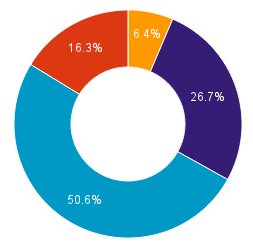
\includegraphics[width=\textwidth]{chart_2}
                \caption{Joren}
        \end{subfigure}%
        \begin{subfigure}[hb]{0.20\textwidth}
                \centering
                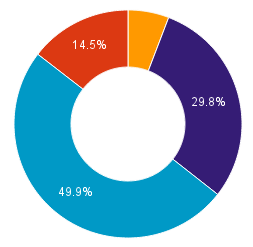
\includegraphics[width=\textwidth]{chart_3}
                \caption{Toon}
        \end{subfigure}%
        \begin{subfigure}[hb]{0.20\textwidth}
                \centering
                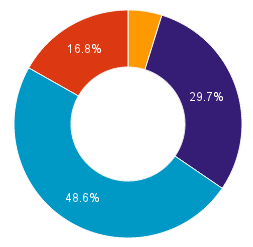
\includegraphics[width=\textwidth]{chart_4}
                \caption{Stef}
        \end{subfigure}%
        \begin{subfigure}[hb]{0.20\textwidth}
                \centering
                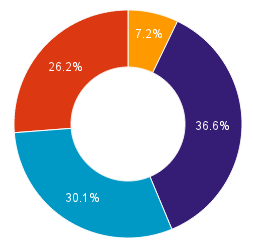
\includegraphics[width=\textwidth]{chart_5}
                \caption{Sophie}
        \end{subfigure}%
                \begin{subfigure}[hb]{0.20\textwidth}
                \centering
                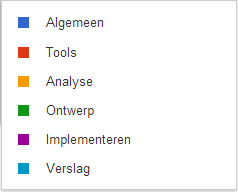
\includegraphics[width=\textwidth]{legende}
                \caption{Legende}
        \end{subfigure}%


 \caption{Weergave van de werkverdeling}
\label{fig:werkverdeling}
\end{figure}





%-----------------------------------------------------------------------
%	 CONCLUSIE en DISCUSSIE
%-----------------------------------------------------------------------
\section{Conclusion and discussion}
\label{ssec:conclusion}
% Een hoofdstuk met een discussie en conclusie waarin interessante ervaringen, problemen en
%andere opmerkingen omtrent het project worden beschreven



%-----------------------------------------------------------------------
%	GLOSSARY
%-----------------------------------------------------------------------
\section{Glossary}
\label{ssec:glossary}


Daemon met een policy en een testinformation Klasse en een Statistic information 

Pattern Model-View-Controller
View:  GUI, CLI, passive view
Controller:
Input besturingsview, handeld input/output
Model: Daemon, Policy, TestInfomation, DataCollector, Statistic, TestRun
Daemon is bedoeld als interface voor het model
\\
Verantwoordelijkheden
Policy: ordening, filtering
Statistic: berekent de statistieken, legt een strategie vast om data op te vragen.
TestInformation:  Houdt de statistieken bij (alles dat uit de collectors wordt opgevraagd)
DataCollector: Data verzameling, inpluggen in een TestRun, change code bijhouden (apart in een andere Collector)
Daemon:  Starten van TestRuns
TestRun:  runnen van testen
\\
Implementaties:
Policy als Composit/Decorator/Strategy
We weten niet zeker of het een composit is want er werd getwijfeld tussen Composit en Decorator Pattern. 
Statistic en DataCollector zijn een Strategy
TestInfomation
Eerst mapte Description met een lijst van tuples. Dit is veranderd naar TestSummary
Map\textless Description,OrderedSet\textless TestSummary\textgreater \textgreater
	TestSummary	-Map\textless Collector, Object\textgreater
			- TestID \\
We streven voor low-coupling. 

Verslag: beginnen met de analyse van wat we nodig hebben en daarna uitleggen hoe we dit oplossen en analyseren en bediscussi\"eren.

 


\end{document}



